%  LaTeX support: latex@mdpi.com
%  In case you need support, please attach any log files that you could have,
% and specify the details of your LaTeX setup (which operating system and LaTeX
% version / tools you are using).

%=================================================================

% LaTeX Class File and Rendering Mode (choose one)
% You will need to save the "mdpi.cls" and "mdpi.bst" files into the same folder
% as this template file.

%=================================================================

\documentclass[energies,article,accept,moreauthors,pdftex,12pt,a4paper]{mdpi}

%=================================================================
\setcounter{page}{1}
\lastpage{x}
\doinum{10.3390/------}
\pubvolume{xx}
\pubyear{2015}
\history{Received: xx / Accepted: xx / Published: xx}
%------------------------------------------------------------------
% The following line should be uncommented if the LaTeX file is uploaded to
% arXiv.org
%\pdfoutput=1

%=================================================================

% Add packages and commands to include here
% The amsmath, amsthm, amssymb, hyperref, caption, float and color packages are
% loaded by the MDPI class.
\usepackage{graphicx}
%\usepackage{subfigure,psfig}
\usepackage[draft]{todonotes}

\def \p{\partial}
\def \d{\mathrm{d}}
\def \D{\mathrm{D}}

%=================================================================
%% Please use the following mathematics environments:
%\theoremstyle{mdpi}
%\newcounter{thm}
%\setcounter{thm}{0}
%\newcounter{ex}
%\setcounter{ex}{0}
%\newcounter{re}
%\setcounter{re}{0}
%\newtheorem{Theorem}[thm]{Theorem}
%\newtheorem{Lemma}[thm]{Lemma}
%\newtheorem{Characterization}[thm]{Characterization}
%\newtheorem{Proposition}[thm]{Proposition}
%\newtheorem{Property}[thm]{Property}
%\newtheorem{Problem}[thm]{Problem}
%\newtheorem{Example}[ex]{Example}
%\newtheorem{Remark}[re]{Remark}
%\newtheorem{Corollary}[thm]{Corollary}
%\newtheorem{Definition}[thm]{Definition}
%% For proofs, please use the proof environment (the amsthm package is loaded by
% the MDPI class).

%=================================================================

% Full title of the paper (Capitalized)
\Title{Effects of Reynolds Number on the Performance and Near-Wake of a
Vertical-Axis Cross-Flow Turbine}

% Authors (Add full first names)
\Author{Peter Bachant $^{1,}$* and Martin Wosnik $^{1}$}

% Affiliations / Addresses (Add [1] after \address if there is only one
% affiliation.)
\address{%
$^{1}$ Center for Ocean Renewable Energy, University of New Hampshire, 24
Colovos Rd., Durham, NH, USA}

% Contact information of the corresponding author (Add [2] after \corres if
% there are more than one corresponding author.)
\corres{pxL3@unh.edu}

% Abstract (Less than 200 words)
\abstract{The acceptable Reynolds number mismatch for scaled physical model
testing a cross-flow turbine is investigated experimentally, both with respect
to prediction of full-scale performance, and wake characteristics, which will be
drivers of overall performance and interaction between multiple turbines.}

% Keywords: add 3 to 10 keywords
\keyword{keyword; keyword; keyword}

% The fields PACS, MSC, and JEL may be left empty or commented out if not
% applicable
%\PACS{}
%\MSC{}
%\JEL{}

\begin{document}

\listoftodos

\section{Introduction}

Scaled physical models are often used in science and engineering to approximate
real-world systems. In the fields of wind and marine hydrokinetic (MHK) energy,
scaled physical models are used to validate numerical models, test prototypes of
individual devices, and design or investigate arrays of devices. Despite being
significantly less expensive, there is still some concern at which scale an
experiment must be performed to be relevant to full-scale application.

For numerical models, one might obtain favorable predictions for scaled systems
due to modified physics. If the numerical model is then considered
``validated,'' there is a risk that its application at full-scale may produce
incorrect predictions. For scaled physical prototypes, it is of interest how
small---since size, or scale generally correlates inversely with cost---the
prototype can be while remaining a reliable predictor of full-scale behavior.

When designing or studying arrays, it is very common to use very small
(geometrically) scaled devices. Sometimes these are not even models of turbines,
but wake generating objects, e.g., porous disks, that are meant to replicate the
wakes of real turbines. In this case, it is of interest to determine at what
scale one might be able to realistically study wake flows in an array, and also
to evaluate the effectiveness of a wake generator, i.e., a wake generator may do
a fine job simulating a scaled turbine, but how well can it simulate a real
turbine?

Previously, Bachant and Wosnik \cite{Bachant2015-JoT} showed that a cross-flow
turbine wake's unique mean flow field is responsible for accelerated wake
recovery when compared with conventional axial-flow propeller-type turbines.

Previously we took a general look at how maximum performance and some 2D wake
profiles are affected by Reynolds number, but here we week to look much deeper.

In this study we set out to measure the effects of scale, both Reynolds and
Froude scales, on the performance of the turbine, and its near-wake
characteristics.

\todo[inline]{Talk about interdependence of Froude number.}

\subsection{Reynolds Number Effects}

In this study we are focused on a turbine constructed from foils---a lift-driven
device in contrast to drag-driven. A logical starting point for understanding
the effects of $Re$ on overall turbine loading is to look at simplified cases
of individual foils, with respect to their static and dynamic loading. 

Chamorro et al. showed that turbulence statistics in an AFT wake became
$Re$-independent at $Re_D \approx 1 \times 10^5$, with mean velocity slightly
earlier at $Re_D \approx 5 \times 10^4$ \cite{Chamorro2012}.

\subsubsection{On Static Foil Behavior}

Turbine performance is strongly dependent on the lift-to-drag ratio $l/d$ acting
on the blades, which is a function of the blades' angles of attack $\alpha$.
These angles of attack are a function of turbine tip speed ratio, induction
(slowing/turning of the free stream flow prior to reaching the turbine), and
turbine rotation or azimuthal angle $\theta$. Looking at static airfoil data, we
see that the static stall angle---the angle just beyond that at which $l/d$ is
maximum, characterized by flow separation near the leading edge---increases with
blade chord Reynolds number $Re_c$. This can be explained as the transition to a
turbulent boundary layer adjacent to the blade delaying separation. However,
static foil performance does not tell the whole story for a cross-flow turbine.
The azimuthal, and therefore temporal variation of $\alpha$ in a cross-flow
turbine implies the occurrence of dynamic stall at tip speed ratios at and below
those of maximum rotor torque\cite{Para2002}. We then must understand the
effects of Reynolds number on the dynamic stall process.

As previously mentioned, the near-wake of a CFT is not very similar to a simple
drag source, or plane shear flow. One of the mean wake's streamwise vortex pairs
can be predicted by potential flow theory as a result of finite-span blades
producing lift (blade end effects), but the other---caused by viscous effects,
i.e., dynamic stall---is not. We can attempt to predict changes
\todo[inline]{Finish this thought with Reynolds number dependence of these
simpler flows, and set up the question whether or not we can assume these will
combine linearly to produce the wake $Re$-dependence we see.}

\begin{figure}[ht]
\caption{Airfoil lift to drag ratio as a function of Reynolds number, from 
\cite{McMasters1980}.}
\end{figure}

\subsubsection{On Dynamic Foil Behavior}

Dynamic effects on blade loading can be distinguished between attached and
separated conditions. 

Bousman showed that dynamic stall was insensitive to Reynolds number for $Re=1.0
\times 10^5$--$2.5 \times 10^5$ \cite{Bousman2000-evaluation}.

\subsubsection{On Wake Flows}

We expect that lower lift on the blades at lower $Re$ will weaken tip vortex
shedding, and decrease the levels of turbulence shed from the blade boundary
layers. As mentioned previously, the dynamic stall vortex shedding is not
expected to have a large Reynolds number sensitivity.

\todo[inline]{What do studies in the literature tell us about $Re$ effects
on shear flows, wakes, and vortex flows?}

\section{Experimental Setup}

Experiments were performed in the University of New Hampshire's tow/wave tank
turbine test bed. The turbine model is dubbed the UNH-RVAT, for Reference
Vertical Axis Turbine, which is designed to be a generic case for numerical
model testing, similar to the Sandia National Labs/US Department of Energy RM2
River Turbine. Details of the turbine and experimental setup are described in
\cite{Bachant2015-JoT}, and a CAD model of the turbine is available from
\cite{Bachant2014-RVAT-CAD}.

\todo[inline]{Make sure to use drawing of turbine with no hubs, since these were
included in the tare drag}


\subsection{Test Plan} 

Approximately 1500 tows were performed, each one used for a single data point on
either a performance curve or wake map. A performance curve consisted of 31
tows, where during each tow the mean turbine tip speed ratio was held constant,
ranging from 0.1--3.1 in 0.1 increments. Full performance curve data were
acquired for tow speeds from 0.4 to 1.2 m/s in 0.2 m/s increments, for which
turbine diameter and approximate blade chord Reynolds number are presented in
Table~\ref{tab:Re}. Performance was also measured for $\lambda=1.9$ at tow
speeds $[0.3, 0.5, 0.7, 0.9, 1.1, 1.3]$ m/s, each of which consisted of two tows.

\begin{table}
\centering
\begin{tabular}{ccc}
Tow speed (m/s) & $Re_D$ & $Re_{c,\mathrm{ave}}$ ($\lambda = 1.9$) \\ 
\hline
0.3 & $3.0 \times 10^5$ & $8.0 \times 10^4$ \\ 
0.4 & $4.0 \times 10^5$ & $1.1 \times 10^5$ \\ 
0.5 & $5.0 \times 10^5$ & $1.3 \times 10^5$ \\ 
0.6 & $6.0 \times 10^5$ & $1.6 \times 10^5$ \\ 
0.7 & $7.0 \times 10^5$ & $1.9 \times 10^5$ \\ 
0.8 & $0.8 \times 10^5$ & $2.1 \times 10^5$ \\ 
0.9 & $0.9 \times 10^5$ & $2.4 \times 10^5$ \\ 
1.0 & $1.0 \times 10^6$ & $2.7 \times 10^5$ \\ 
1.1 & $1.1 \times 10^6$ & $2.9 \times 10^5$ \\ 
1.2 & $1.2 \times 10^6$ & $3.2 \times 10^5$ \\ 
1.3 & $1.3 \times 10^6$ & $3.4 \times 10^5$ \\ 
\end{tabular} 
\caption{Turbine diameter and approximate blade chord Reynolds numbers for the
tow speeds used in the experiment.}
\label{tab:Re}
\end{table}

A wake map was generated by positioning a Nortek Vectrino+ acoustic Doppler
Velocimeter (ADV) at 270 different locations, varied in the cross-stream and
vertical directions at one turbine diameter downstream. These locations have
vertical coordinates from the turbine centerline up to $z/H=0.625$, ranging in
the cross-stream direction $y/R = \pm 3$. These locations are shown in
Figure~\ref{fig:wake-locations}.

\begin{figure}
\centering
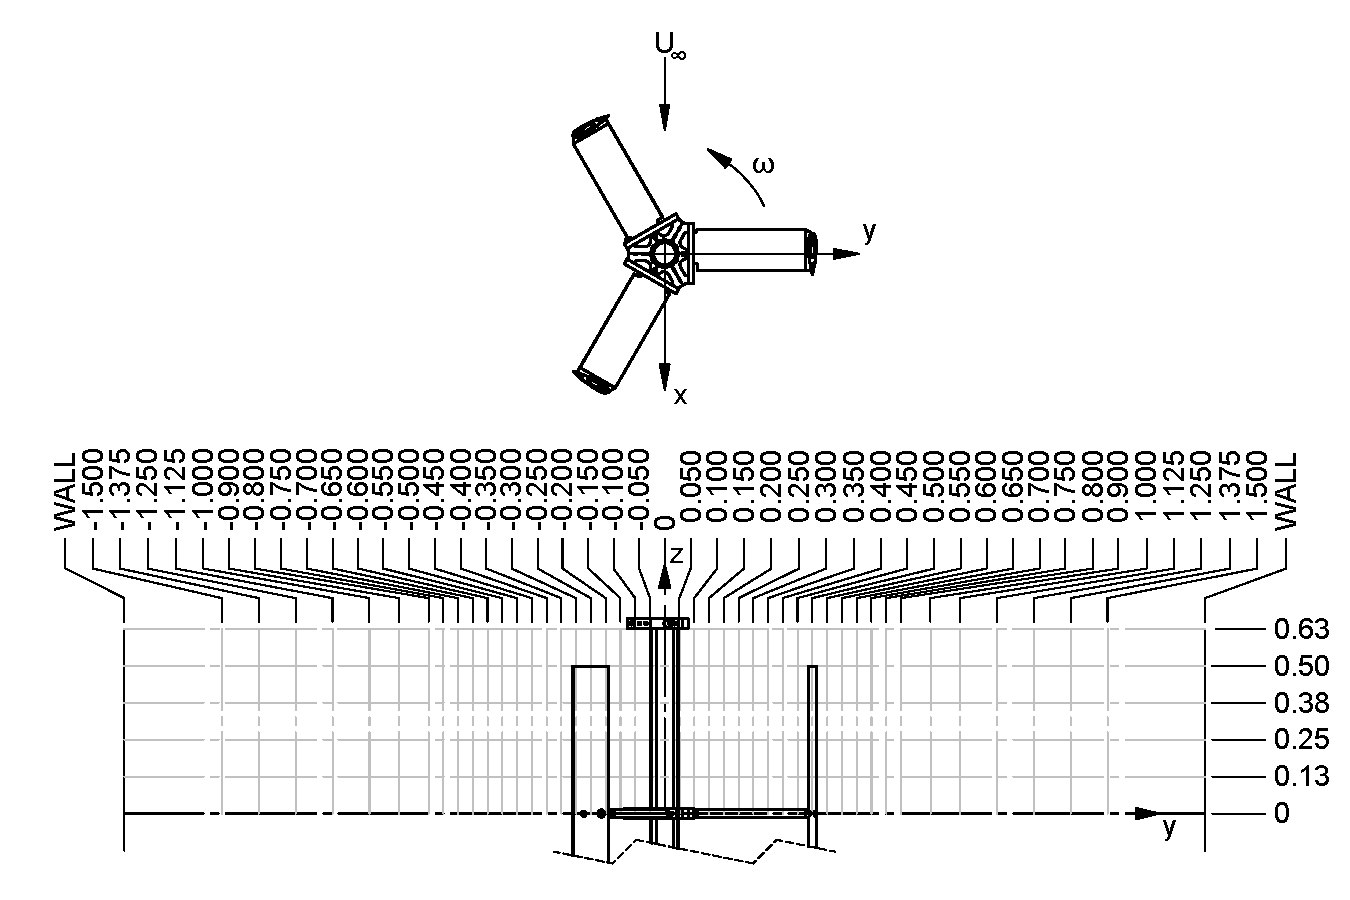
\includegraphics[width=0.9\textwidth]{figures/turbine_coordinate_system}
\caption{Wake measurement coordinate system and locations. Dimensions are in
meters.} 
\label{fig:wake-locations}
\end{figure}

\subsection{Data Processing}

From each set of tows, a standard time interval was set, and each run was
analyzed to compute statistics over this interval, truncating the end slightly
to achieve and integer number of blade passages.

\todo[inline]{Cite reduced data and processing code on figshare.}


\section{Results and Discussion}


\subsection{Performance}

Full performance curves for various Reynolds numbers are plotted in
Figure~\ref{fig:perf-curves}. There is essentially no change in the shape of the
drag coefficient curves---merely an upward shift in $C_D$ with increasing $Re$.

In general, maximum $C_P$ increases with Reynolds number, which is due to an
increase in the foil lift-to-drag ratio. The power coefficient curves also show
a downward shift in the optimal tip speed ratio with increasing Reynolds number.
This is caused by the stall delay from a more turbulent boundary later on the
blade suction side.

\begin{figure}[ht]
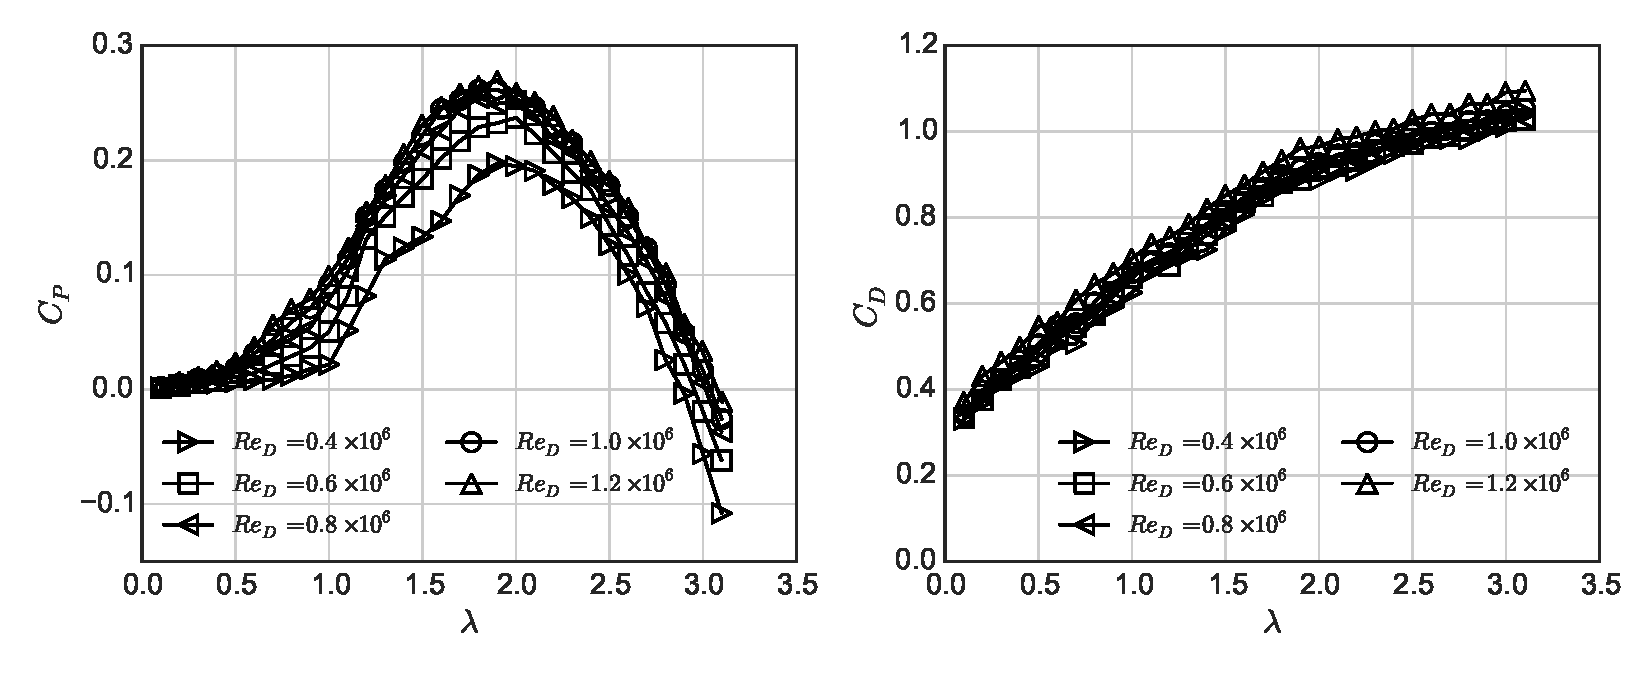
\includegraphics[width=0.95\textwidth]{figures/perf_curves}
\caption{Mean power (left) and drag (right) coefficient curves plotted for
multiple Reynolds numbers.}
\label{fig:perf-curves}
\end{figure}

Mean power and drag coefficients at $\lambda=1.9$ are plotted for all Reynolds
numbers in Figure~\ref{fig:perf-Re-dep}. There is a drastic improvement in $C_P$
with increasing Reynolds number for the lower values. Power coefficient then
becomes  essentially $Re$-independent at $Re_D = 0.8 \times 10^6$, which
corresponds to an approximate average blade chord Reynolds number $Re_{c,
\mathrm{ave}} = 2.1 \times 10^5$. This threshold is consistent with the behavior
of the blade boundary layer transitioning from laminar to turbulent, thereby
promoting reattachment of the laminar separation bubble.

The behavior of the mean rotor drag coefficient is similar, though the changes
are less dramatic. This is likely due to cross-flow turbine geometry, where
increases in blade drag at lower $Re$ somewhat offset the reduction in lift, to
keep total streamwise force from changing as much as the rotor torque. The
tendency for $C_D$ to continue increasing with $Re$ may also be a consequence of
increasing Froude number, which therefore increases free surface deformation and
wave drag during towing without increasing flow through the turbine.

\begin{figure}[ht]
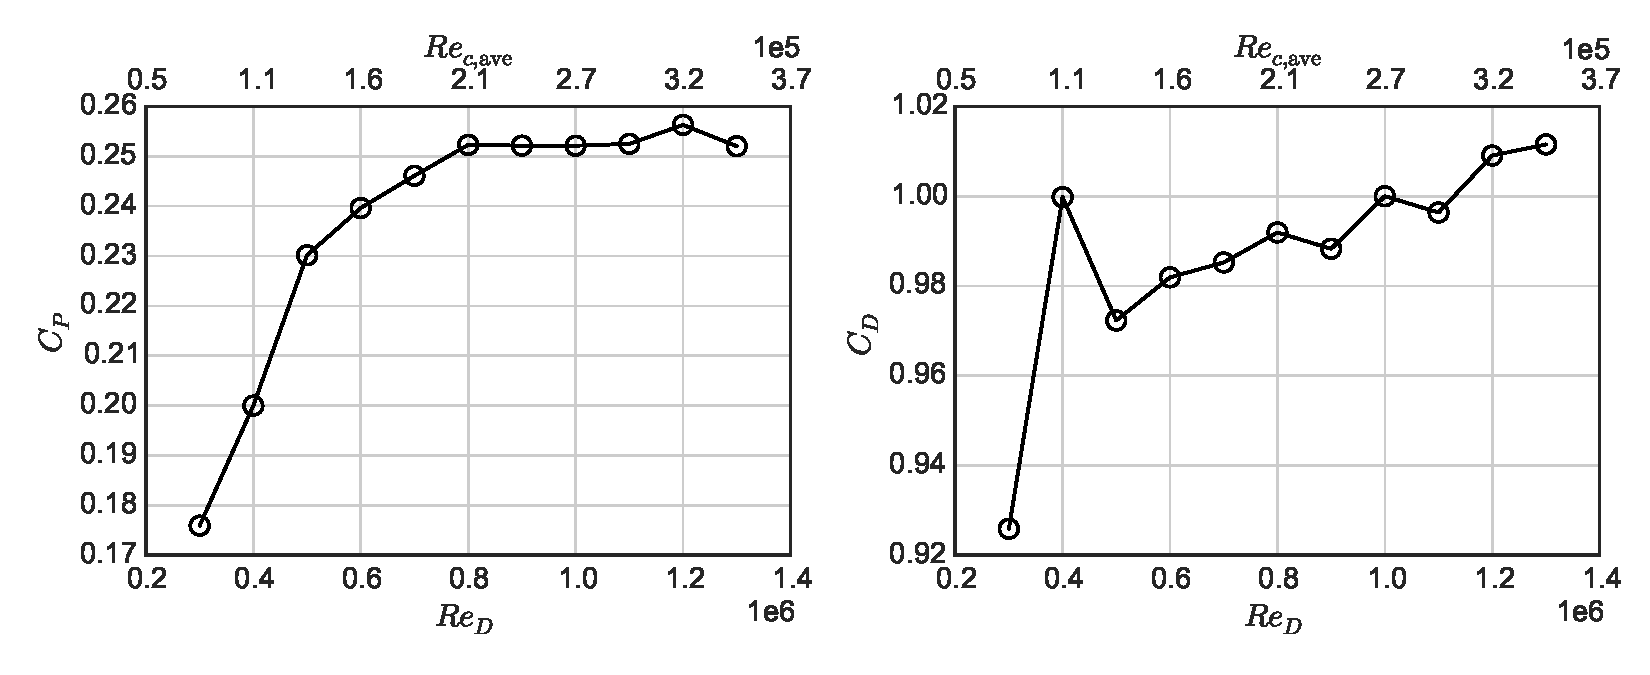
\includegraphics[width=0.95\textwidth]{figures/perf_re_dep}
\caption{Mean power (left) and drag (right) coefficients at $\lambda=1.9$
plotted versus Reynolds number.} 
\label{fig:perf-Re-dep}
\end{figure}

\subsubsection{Understanding via Static Foil Coefficients}

To help understand---and possibly predict---the $Re$-sensitivity on turbine
performance, a series of foil coefficient datasets were computed with the XFOIL
viscous panel method code.

The turbine torque coefficient $C_T$ can be related to the blade section
chordwise force coefficient $C_c$ by
\begin{equation}
C_T = \frac{C_c c}{2R} \frac{|U_\mathrm{rel}|^2}{U_\infty^2},
\end{equation}
where the blade section chordwise force (for zero preset pitch)
\begin{equation}
C_c = C_l \sin \alpha - C_d \cos \alpha.
\end{equation}

\begin{figure}[ht]
\centering
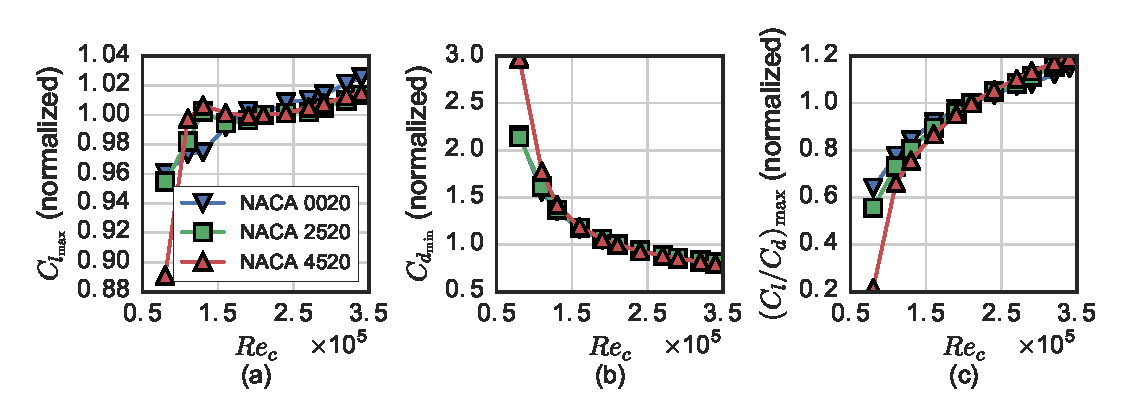
\includegraphics[width=0.95\textwidth]{figures/all_foils_re_dep}
\caption{Foil section characteristics computed by XFOIL for various $Re_c$.}
\label{fig:foil-Re-dep}
\end{figure}

\begin{figure}[ht]
\centering
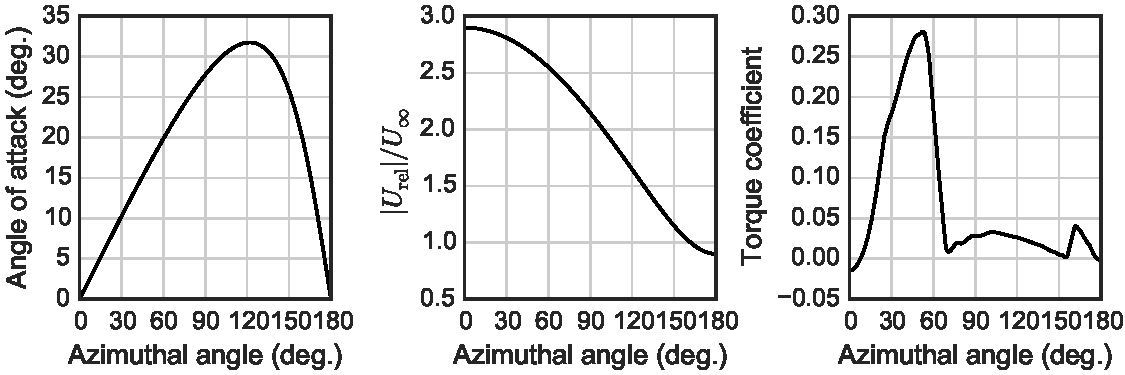
\includegraphics[width=0.95\textwidth]{figures/foil_kinematics_ct}
\caption{Geometric angle of attack (a), relative velocity (b) and torque coefficient
(c) calculated with a NACA 0020 foil.}
\label{fig:blade-kinematics}
\end{figure}

\begin{figure}[ht]
\centering
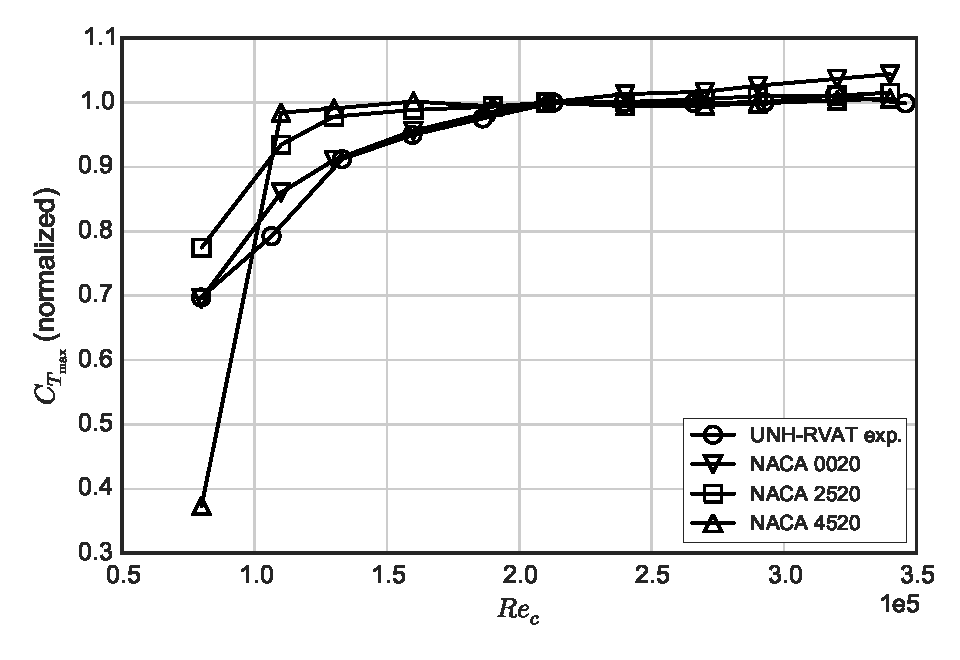
\includegraphics[width=0.65\textwidth]{figures/cft_re_dep_foils}
\caption{Reynolds number dependence of the peak torque coefficient calculated using 
only static foil coefficients and blade kinematics.}
\label{fig:foils-C_T-Re-dep}
\end{figure}

Note that the common static foil performance metrics fail to show Reynolds
number dependence as close as the max geometric torque coefficient. This means
that the turbine kinematics play an important role, even if the exact dynamics
of the flow are not known.

\subsection{Wake Characteristics}

\todo[inline]{Put wake characteristics here. Maybe create difference plots to
show absolute differences, or RMS, or something}


\todo[inline]{Plot asymptotic behavior for a bunch of locations all on the same
plot.}



\subsubsection{Dominant Timescales}

\todo[inline]{Look at how spectra change when turbine rotational frequency
changes relative to inertial subrange.}

\begin{figure}[ht]
\centering
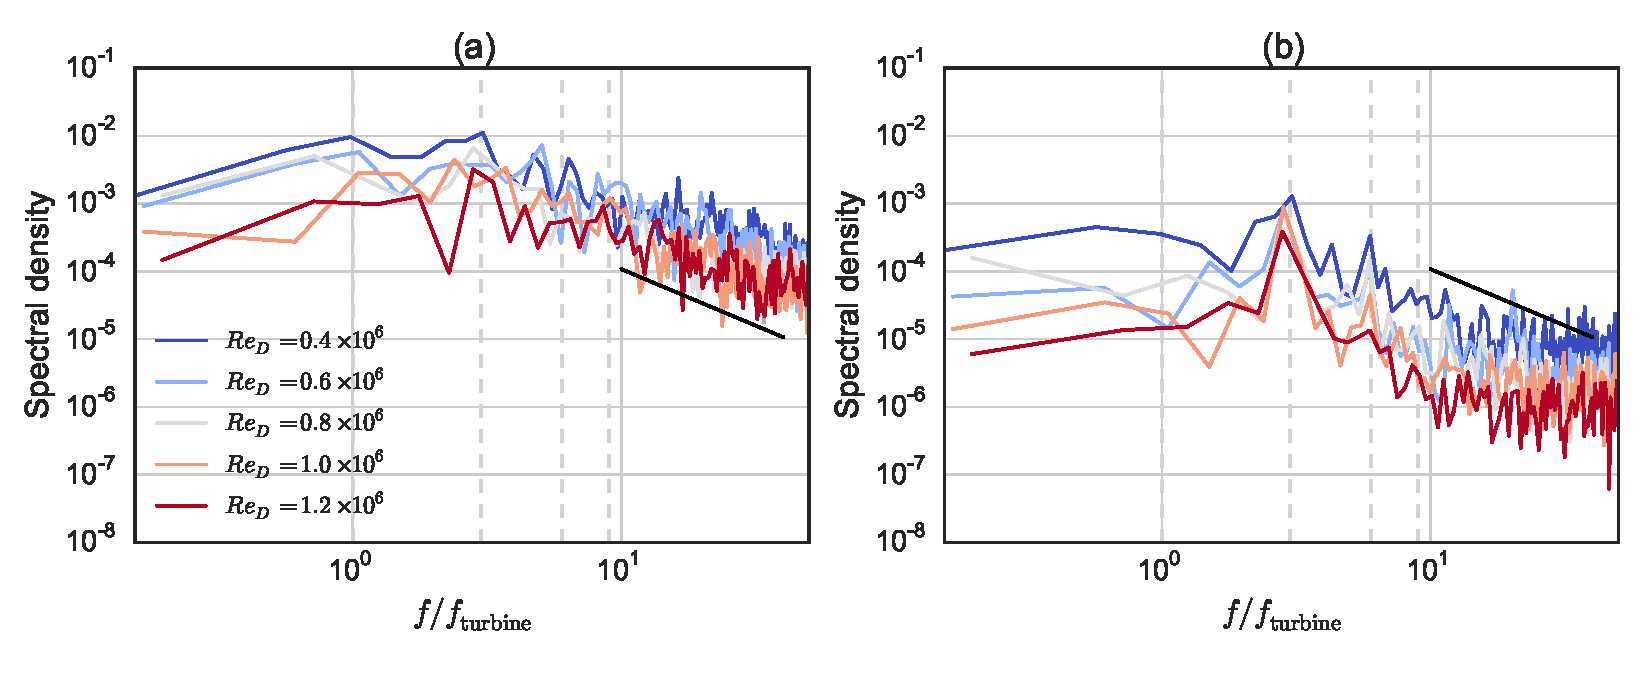
\includegraphics[width=0.95\textwidth]{figures/wake_spectra}
\caption{Wake spectra at $z/H=0.25$, $y/R=-1.0$ (a) and $y/R=1.5$ (b). Dashed vertical
lines indicate $[1, 3, 6, 9]$ times the turbine rotational frequency.}
\label{fig:wake-spectra}
\end{figure}



\subsubsection{Mean Momentum and Kinetic Energy Transport}


\begin{figure}[ht]
\centering
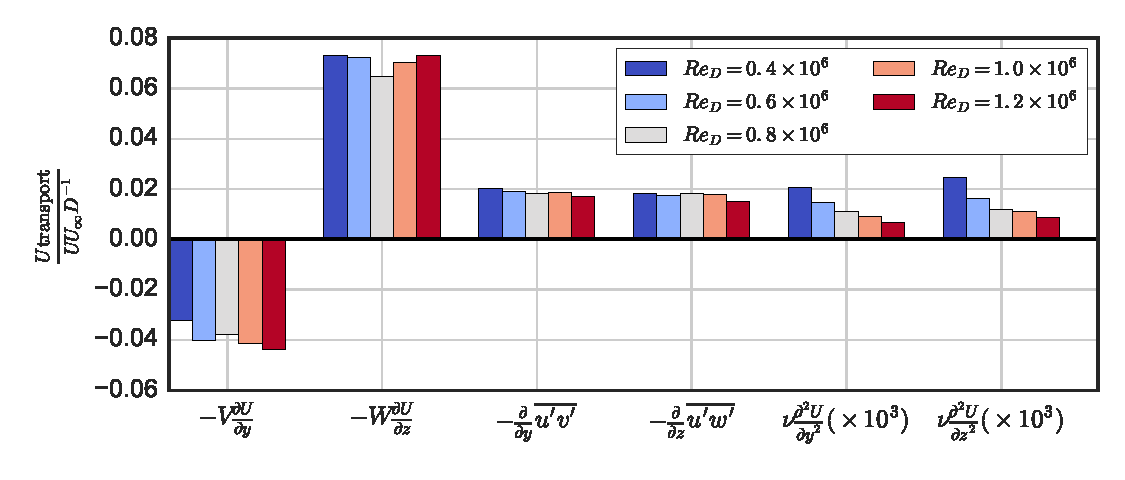
\includegraphics[width=0.9\textwidth]{figures/mom_bar_graph}
\caption{Momentum transport quantities.}
\label{fig:mom-bar-graph}
\end{figure}


The relative importance of various physical processes on mean kinetic energy
transport/recovery in the streamwise direction $\p K / \p x$ are plotted in...

\begin{figure}[ht]
\centering
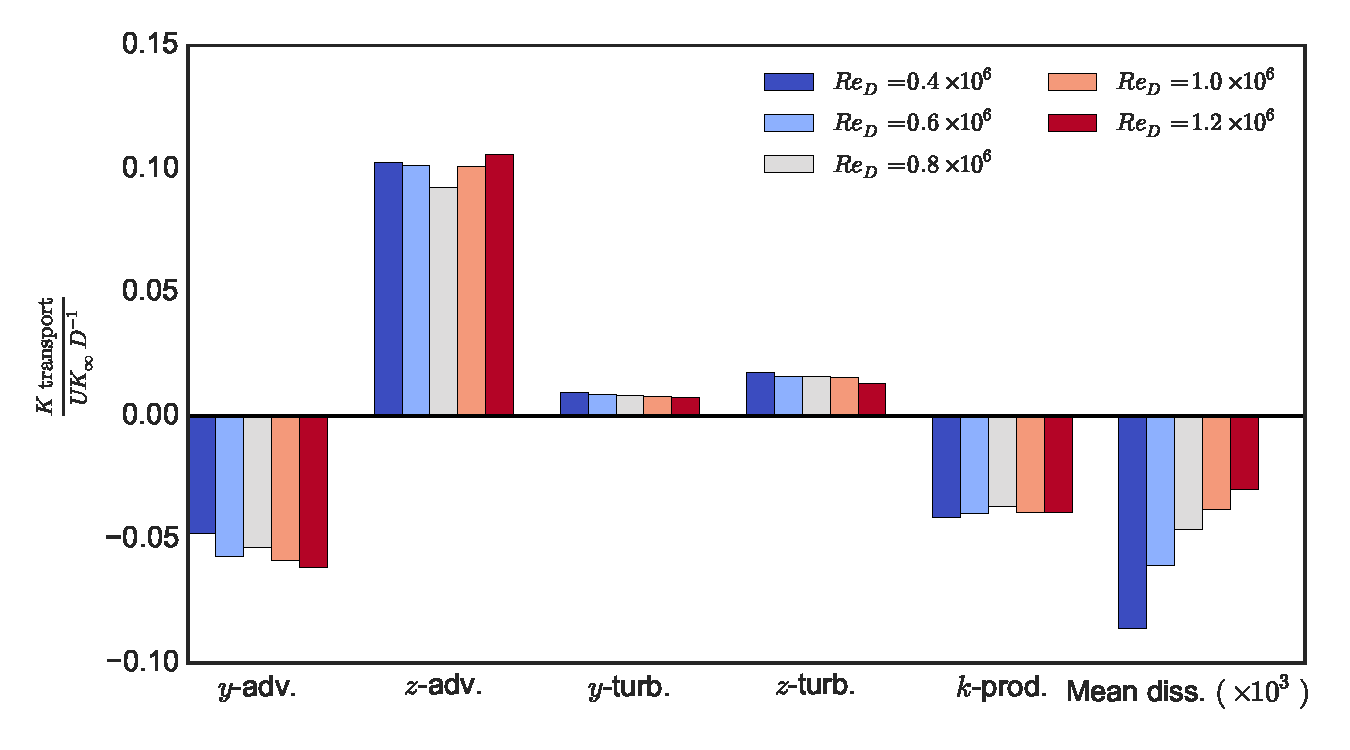
\includegraphics[width=0.9\textwidth]{figures/K_trans_bar_graph}
\caption{Mean kinetic energy transport quantities.}
\label{fig:K-bar-graph}
\end{figure}


\begin{figure}[ht]
\centering
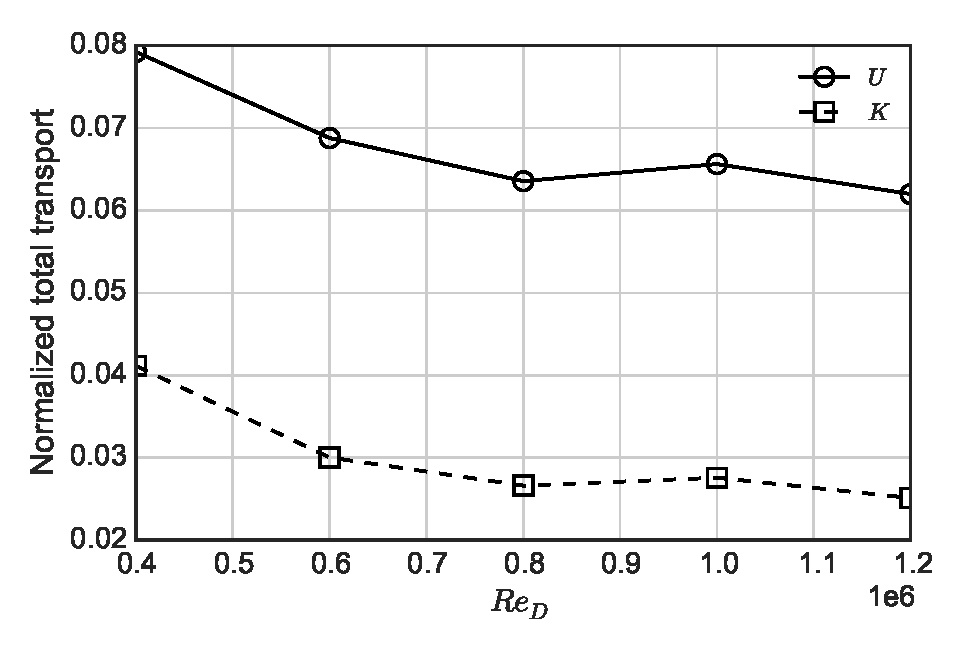
\includegraphics[width=0.65\textwidth]{figures/wake_trans_totals}
\caption{Normalized transport totals from Figures~\ref{fig:mom-bar-graph} and 
\ref{fig:K-bar-graph} plotted versus Reynolds number.}
\label{fig:wake-trans-totals}
\end{figure}


\section{Conclusions}

In this study we determined that, as previously shown, turbine performance
becomes essentially $Re$-independent at a turbine diameter Reynolds number $Re_D
\approx 10^6$, or an approximate blade chord Reynolds number $Re_c \approx 2
\times 10^5$.

These results suggest that to validate predictive engineering models, one must
use data of at least this scale, especially high-fidelity CFD models, where
transition to turbulence may be completely different between scaled physical
model and prototype.

If using scaled physical models to predict array performance, it is important to
keep all turbines in the linear regime to avoid exaggerated power deficiencies
for downstream turbines, despite similarities in wake characteristics

\acknowledgements{Acknowledgements}

The authors would like to acknowledge funding through a National Science
Foundation CAREER award (PI Wosnik, NSF-CBET 1150797, program manager Dr. Ram
Gupta), a grant through the Leslie S. Hubbard Marine Program Endowment to
purchase acoustic flow measurement instrumentation, and a grant for laboratory
infrastructure upgrades through the US Department of Energy.

\conflictofinterests{Conflicts of Interest}

The authors declare no conflict of interest.


\bibliography{library}
\bibliographystyle{mdpi}

\end{document}


